\chapter{Experiments}\label{ch:experiments}

The same cINN normalizing flow architecture, spectral-normalized GAN (SN-GAN)~\cite{sngan} discriminator architecture, and
Adam optimizer parameters between all experiments.
The details of the common model and optimizer hyperparameters are listed in Appendix~\ref{ch:model-and-optimizer-hyperparameters}.
The dataset is split into 2019 and 2020 solely for training and 2021 is held out for evaluation.
A strict backtesting procedure is followed, where a model producing forecasts for an upcoming market-day has only been
trained on data that would be available to a real participant prior to the market-day.

All models in this work were trained on an NVIDIA GTX 1060--6GB GPU using Python v3.10.8 and PyTorch v1.13.0.
While GPU training allowed larger batch sizes and accelerated training times, often under 10 minutes, these
models can be trained on CPU with smaller batch sizes, often taking between 10-30 minutes (tested on an AMD
Ryzen 3700x @ 3.6GHz with 16GB RAM and a 2020 Intel i7 @ 2.3GHz 13-inch Apple Macbook-Pro with 16GB RAM).

\section{Capturing Non-Stationary Prices}\label{sec:capturing-non-stationary-prices}

Changes in market fundamentals over time lead to non-stationary price distributions, with key factors including:
\textit{grid topology}, \textit{fuel prices}, \textit{population and load patterns}, \textit{generator outages},
\textit{renewable penetration}, \textit{generation mix}, \textit{weather patterns}, etc.
Much of the variation in energy prices can be explained by changes in the fundamentals of the dataset,
for example, the relationship between energy prices and gas prices as shown in Figure.~\ref{fig:price_gas_hist},
seasonal load patterns as shown in Figure~\ref{fig:weekly_load}, or seasonal generation mixes shown in
Figure~\ref{fig:weekly_windgen}.
However, while a well-calibrated model can capture the complex, nonlinear relationships of these quantities with the
powerful capacities provided by deep learning methods, these interactions change over time, and with respect to
inaccessible quantities such as grid topology.
Thus, energy price forecasting methods must accurately track the non-stationary distributions and quickly adapt as
new data becomes available.
For the experiments in this section note $\lambda_{\text{ADV}} = 0$.

\begin{figure}[htbp]
    \caption[Quarterly aggregated day-ahead prices v.s. natural gas spot prices]{
        Quarterly distributions of Chicago Hub DA-LMPs and natural gas spot prices over time.
        The left-y-axis and histograms show the distribution of Chicago Hub DA-LMPs aggregated
        quarterly.
        The right-y-axis and black dots-and-flyers show quarterly aggregate natural gas prices at TETCO-M3
        where the dots represent the mean price. The upper and lower flyers represent the $75^{\text{th}}$ and
        $25^{\text{th}}$ percentiles respectively.
    }
    \begin{center}
        \setlength{\fboxsep}{0pt}%
        \setlength{\fboxrule}{1pt}%
%        \fbox{
        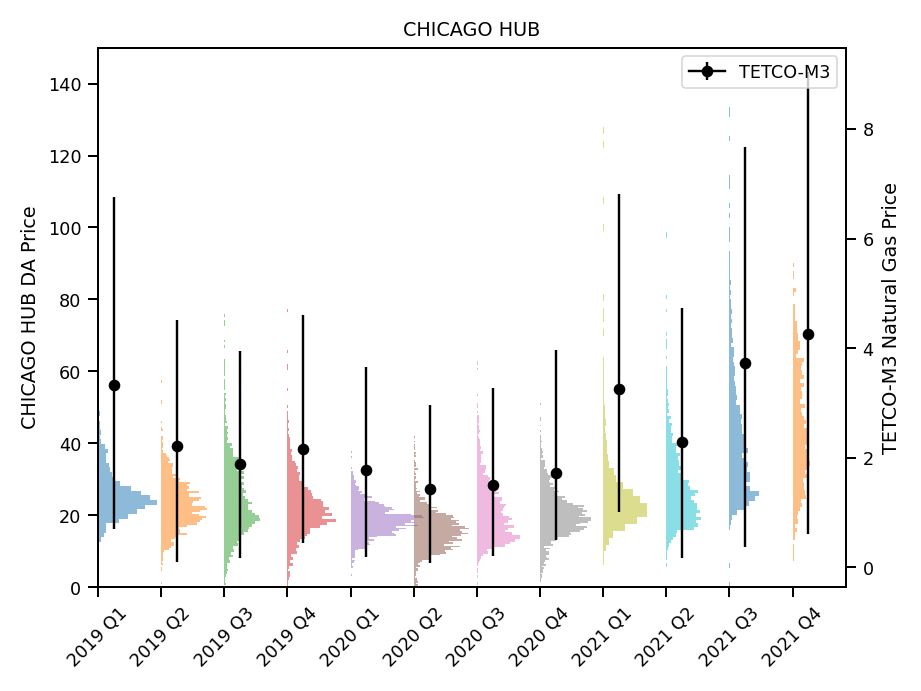
\includegraphics[width=120mm]{figs/chicago_hub_tetco_dists}
%        }
    \end{center}
    \label{fig:price_gas_hist}
\end{figure}

\begin{figure}[htbp]
    \caption[Total aggregate load v.s. day-ahead prices]{
        Weekly averaged Chicago Hub DA-LMPs v.s. PJM total load forecasts.
        The left-y-axis and blue curve show the total load forecast in PJM averaged weekly.
        The right-y-axis and orange curve show the Chicago Hub DA-LMP averaged weekly.
    }
    \begin{center}
        \setlength{\fboxsep}{0pt}%
        \setlength{\fboxrule}{1pt}%
%        \fbox{
        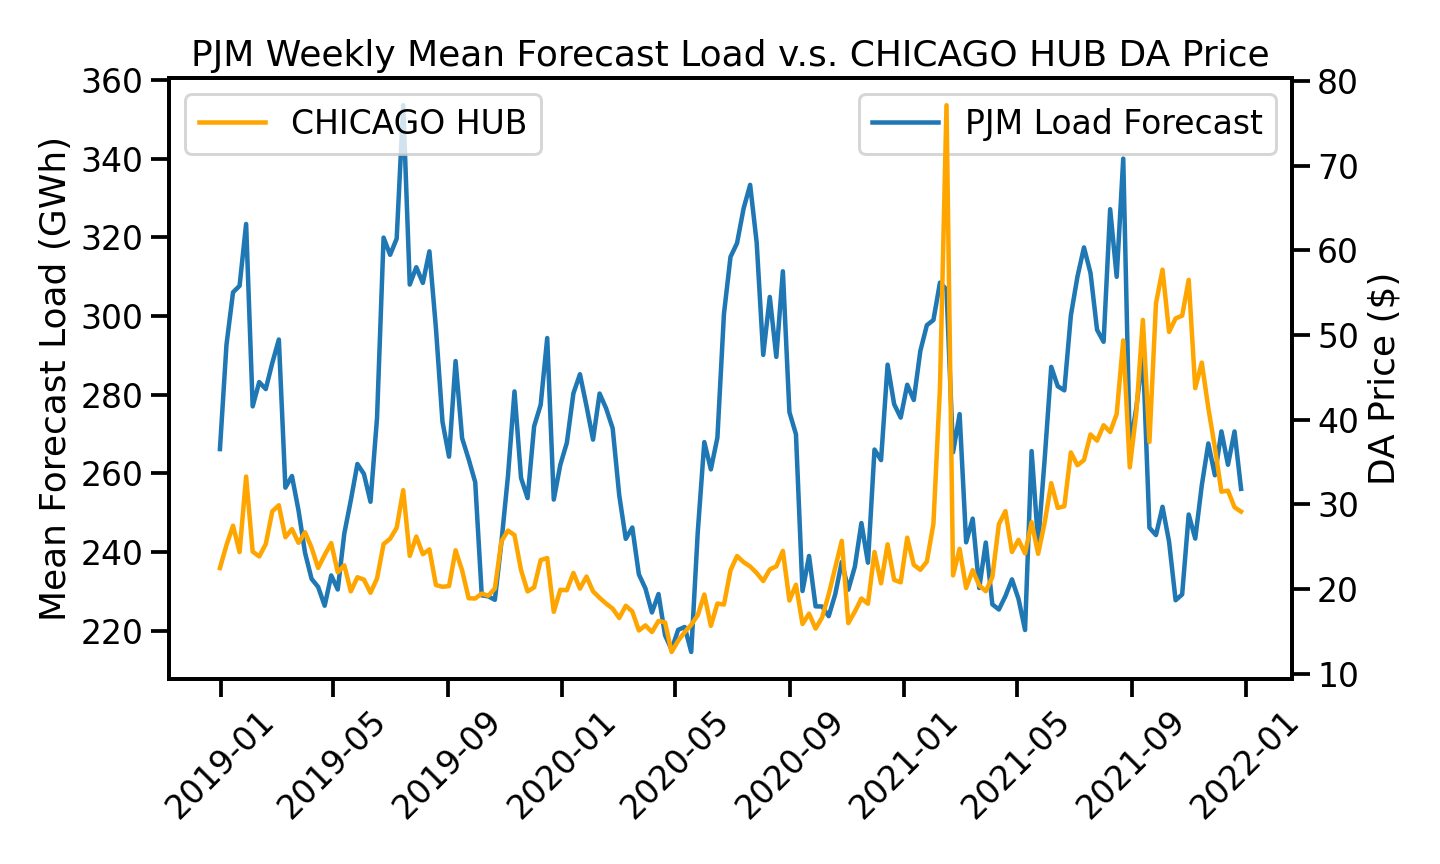
\includegraphics[width=120mm]{figs/load_vs_price}
%        }
    \end{center}
    \label{fig:weekly_load}
\end{figure}

\begin{figure}[htbp]
    \caption[Total aggregate wind generation v.s. day-ahead prices]{
        Weekly averaged Chicago Hub DA-LMPs v.s. PJM total wind generation forecasts.
        The left-y-axis and blue curve show the total wind generation forecast in PJM averaged weekly.
        The right-y-axis and orange curve show the Chicago Hub DA-LMP averaged weekly.
    }
    \begin{center}
        \setlength{\fboxsep}{0pt}%
        \setlength{\fboxrule}{1pt}%
%        \fbox{
        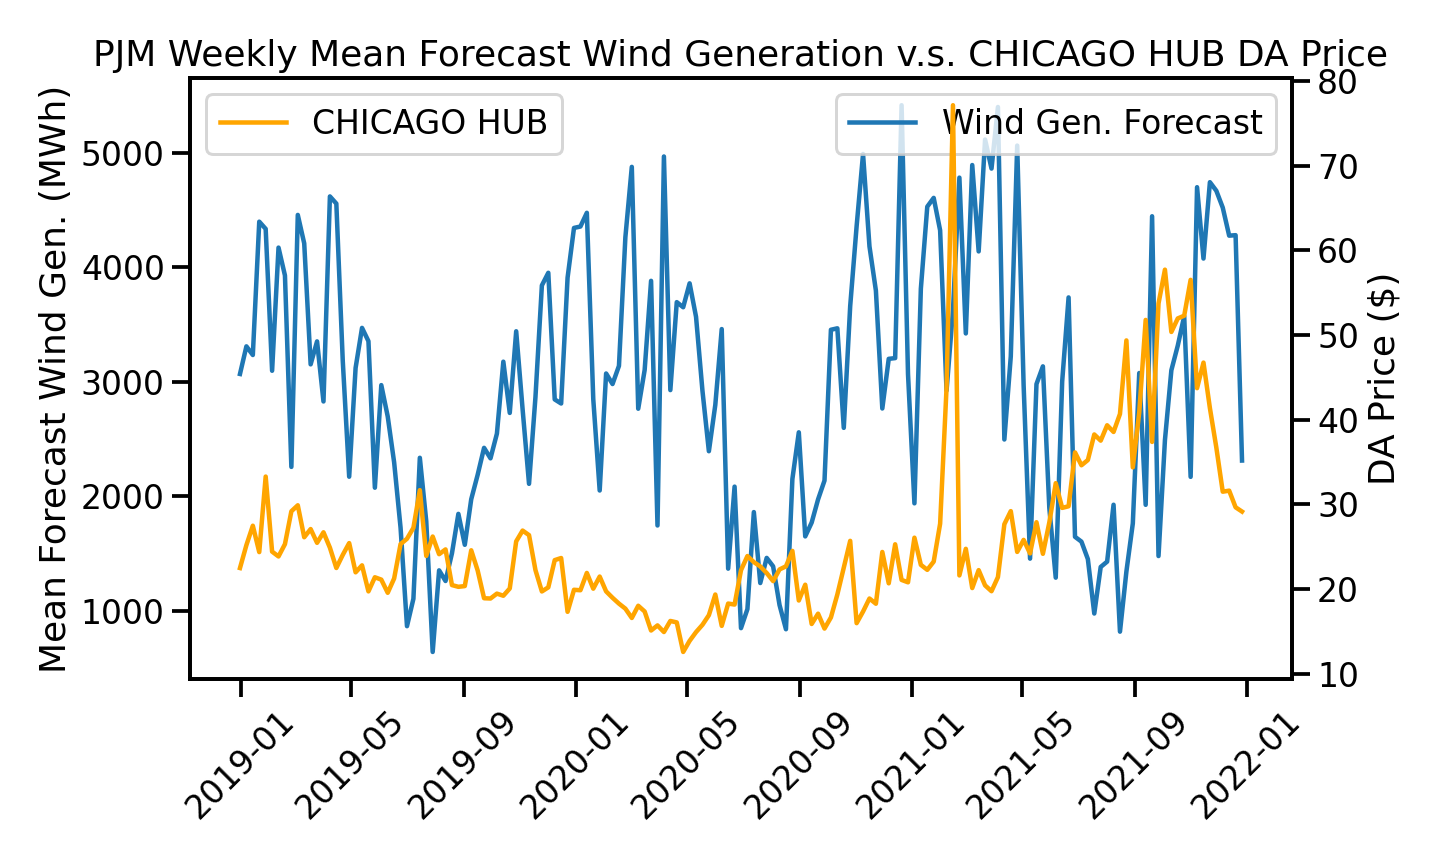
\includegraphics[width=120mm]{figs/windgen_vs_price}
%        }
    \end{center}
    \label{fig:weekly_windgen}
\end{figure}

The following three strategies are proposed for increasing the forecasting skill on non-stationary energy
market data:
\begin{enumerate}
    \item \textbf{Parameter recalibration.} Parameter recalibration (PR) is a common tool used in timeseries
    forecasting whereby after some amount of time has passed and new data
    has become available the parameters of the forecasting model are updated
    using the new observations.
    Let $T \in \mathbb{N}^+$ be a hyperparameter representing the number of
    market-days between recalibrations.
    The model will produce a set of forecasts for a single $T$-day interval
    using fixed parameters, after which, the observations in the $T$-day
    interval are added to the training set and the model is re-trained from
    scratch on the extended history.
    $T=1$ is equivalent to re-training the model from scratch each day before
    trade submission while $T \geq 365$ is equivalent to never recalibrating
    over the entirety of 2021.
    \item \textbf{Rolling training windows.} Rolling training data windows (RT) are another common timeseries
    forecasting tool when old data is assumed to be ``less predictive'' than
    the most recent data.
    Instead of extending the training data by appending new observations to
    history, the size of the training dataset remains fixed and only the most
    recent observations are held for training.
    Let $R \in \mathbb{N}^+$ be a hyperparameter representing the number of
    market-days in the rolling training window.
    When combined with a recalibration interval of $T$ days, after forecasting
    is complete the most-recent observations from the new $T$-day interval
    replace the oldest training observations and the model is trained from
    scratch on the reduced history.
    \item \textbf{Rolling fine-tuning windows.} Rolling fine-tuning windows (FT) extend the idea of rolling training
    windows, however, without reducing the size of the training dataset.
    Let $R \in \mathbb{N}^+$ be a hyperparameter representing the number of
    market-days in the rolling fine-tuning window.
    Just like in parameter recalibration, forecasts are produced for
    $T$-day intervals whose observations are then appended to the training
    data before the model is re-trained from scratch.
    However, after the initial round of training the model is fine-tuned by
    reducing the learning rate and briefly continuing training on a subset
    of the most recent $R$-days in the extended history.
\end{enumerate}

These updating methods are compared against a baseline with parameters that are trained once and never updated with
results in Table~\ref{tab:nonstat}.
Parameter recalibration is shown to improve forecasting skill as the recalibration frequency increases, suggesting that
the most recent market data is substantially more predictive than older observations.
This observation, coupled with short training times, makes the daily recalibration of this model a practical
recommendation.
Inclusion of rolling training data windows with parameter recalibration is shown to negatively impact forecasting
performance, with smaller training window sizes causing substantial degradations.
This is likely caused by overfitting on the smaller training windows leading to reduced out-of-sample performance.
Use of the fine-tuning strategy, however, greatly improves performance.
Observing mCRPS metrics, reducing the fine-tuning window size yields more accurate forecasts, which is likely explained
by the fine-tuning emphasizing relevant (in this case the mose recent) historical observations and further
suggests that the most recent data has the most predictive power.
We believe further refinement of the fine-tuning methodology, in terms of identifying and selecting the ``most
relevant'' data points aside from those most recently observed, can likely lead to more performance gains.

\begin{table}[htb]
    \caption[Comparison of strategies for handling non-stationary data]{
        Evaluation metrics comparing methodologies to handle non-stationary data.
    }
    \begin{center}
        \begin{tabular}{||c|c|c|c||} \hline
        Update Method & Median NLL (-)  & $99\%$ NLL (-) & mCRPS (-)  \\	% footnote symbols!
        \hline \hline
        None                         &         -26.337  &         86.574  &        10.392  \\ \hline
        PR ($T = 90$)                &         -41.724  &         65.773  &         9.413  \\
        PR ($T = 14$)                &         -44.127  & \textbf{63.294} &         7.508  \\ \hline
        PR + RT ($T = 14$, $R = 90$) &         -47.907  &        283.582  &         8.327  \\
        PR + RT ($T = 14$, $R = 14$) &          25.551  &     418573.25   &        15.43   \\ \hline
        PR + FT ($T = 14$, $R = 45$) & \textbf{-52.346} &         66.59   &         6.686  \\
        PR + FT ($T = 14$, $R = 14$) &         -49.839  &         65.27   & \textbf{5.723} \\ \hline
        \end{tabular}
        \\ \rule{0mm}{5mm}
    \end{center}
    \label{tab:nonstat}
\end{table}

\section{Improving Sampling Tasks with Adversarial Loss}\label{sec:improving-sampling-tasks}

Next, the impact of including the adversarial loss term, $\mathcal{L}_{\text{ADV}}$, in the hybrid loss function and
how it specifically affects the sampling performance of the model are investigated.
The aforementioned 14-day recalibration and 14-day fine-tuning window methods are utilized in the following experiments.
A range of values for $\lambda_{\text{ADV}} > 0$ are swept over and compared against a baseline model without adversarial
loss with results shown in Table~\ref{tab:ganloss}.

\begin{table}[htb]
    \caption[Results of adversarial loss inclusion]{
        Comparison of fine-tuning rolling window sizes
    }
    \begin{center}
        \begin{tabular}{||c|c|c|c||} \hline
        $\lambda_{\text{ADV}}$ & Median NLL (-)  & $99\%$ NLL (-) & mCRPS (-)  \\	% footnote symbols!
        \hline \hline
        0   &         -49.839  &         65.27   &         5.723 \\ \hline
        0.1 &         -50.02   &         65.103  &         5.637 \\ \hline
        1   & \textbf{-50.442} &         65.176  &         5.569 \\ \hline
        10  &         -50.394  & \textbf{62.854} & \textbf{5.309} \\ \hline
        \end{tabular}
        \\ \rule{0mm}{5mm}
    \end{center}
    \label{tab:ganloss}
\end{table}
The inclusion of adversarial loss improves the mCRPS metric.
To investigate why, first recall the definition of the CRPS estimator~\eqref{eq:crps_int} and note the sensitivity of the
CRPS estimator to outliers samples.
Consider the empirical c.d.f for an arbitrary distribution represented by a set of finite samples, if some samples
are extreme outliers then they will carry a non-trivial mass under the tail of the distribution.
Depending on the number and magnitude of the outliers this tail may over-estimate the tail of the true distribution
resulting in a degraded CRPS estimation.

To illustrate this issue with an example, let $\mathcal{U} \sim \text{Gumbel}(\mu=0, \beta=1)$ with realizations $u$.
The empirical c.d.f. $\hat{F}_\mathcal{U}$ is constructed by drawing 500 samples.
A second c.d.f. $\hat{F}'_\mathcal{U}$ is constructed using the same examples, however, with a single outlier observation
$u=10,000$ added to the set of samples.
For an observation at $y=0$, the CRPS estimators are computed to be $\widehat{CRPS}_{\hat{F}_\mathcal{U}}(0) = 0.3331$
and $\widehat{CRPS}_{\hat{F}'_\mathcal{U}}(0) = 0.3748$ respectively.
Clearly, extreme outliers have a detrimental effect on estimated CRPS metrics.

When observing the sample distribution drawn from a trained price density model, extreme outliers are not uncommon.
Figure~\ref{fig:badsamples} shows 500 samples that estimate the joint density forecast between two price nodes
marginalized out from a larger joint forecast.
Most samples are indistinguishable from one another and located near the origin as expected, however,
observe the small number of samples whose magnitudes are on the order of \$$10^7$.
It is clear how these samples would severely degrade the CRPS metrics of this forecast.

\begin{figure}[htbp]
    \caption[Samples drawn joint density forecast with extreme outliers]{
        Samples from a marginalized joint distribution forecast between WESTERN HUB and AEP GEN HUB price nodes.
        Note the outliers with values on the order of magnitude of \$$10^7$ which exceed both
        reasonable price expectations and hard price limits enforced by PJM.
    }
    \begin{center}
        \setlength{\fboxsep}{0pt}%
        \setlength{\fboxrule}{1pt}%
%        \fbox{
        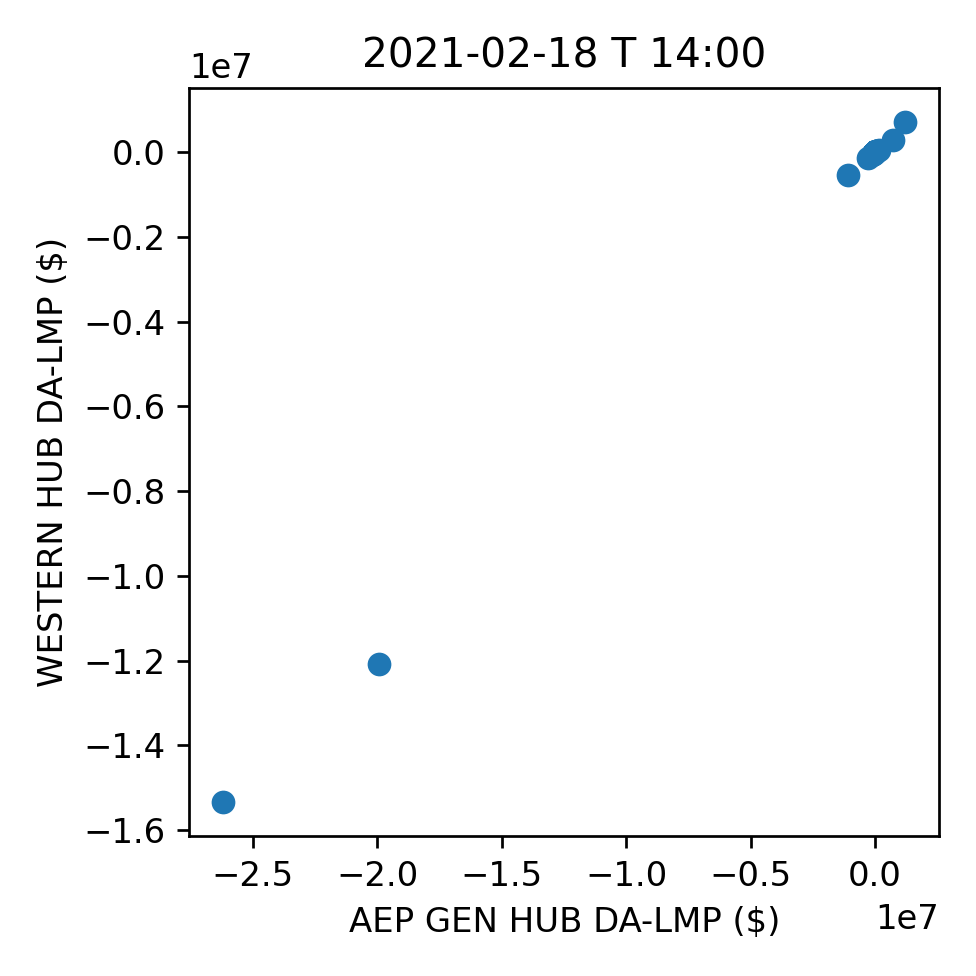
\includegraphics[width=100mm]{figs/bad_samples}
%        }
    \end{center}
    \label{fig:badsamples}
\end{figure}

To determine if adversarial loss address this problem specifically, it is necessary to quantify the frequency of extreme
outliers.
Starting with the matrix $\mathbf{X}_t \in \mathbb{R}^{r \times n}$ representing $r$ samples for a forecast at time
$t$ over $n$ price nodes.
The sample covariance matrix for $\mathbf{X_t}$ associated eigenvalues ${\sigma_1 \dots \sigma_n}$ are computed.
Let the \textit{total uncertainty} (TU) of our forecast be defined as

\begin{equation*}
    \text{TU}_\mathbf{X_t} = \sum_{i=1}^{n} \sqrt{\sigma_i},
    \label{eq:total_uncertainty}
\end{equation*}
which can be interpreted as the cumulative standard deviations in price along each orthogonal dimension in some rotated
price space.
Next, the \textit{excess uncertainty} (EU) is defined as a binary indicator on the total uncertainty exceeding a set
threshold,

\begin{equation*}
    \text{EU}_{\mathbf{X}_t} = \mathbbm{1}_{\left[ TU_{\mathbf{X}_t} \geq 1000 \right]},
    \label{eq:excess_unc}
\end{equation*}
where 1000 is chosen as the threshold because day-ahead prices rarely exceed the low hundreds of dollars on more than a
handful of nodes at any time, thus this threshold is expected to be rarely exceeded under normal market conditions.
Counting the total excess uncertainty over all forecasts on the validation set then provides a metric for the
frequency of outliers,

\begin{equation*}
    \text{Total Excess Uncertainty} = \sum_{t=1}^{T} EU_{\textbf{X}_t}.
    \label{eq:total_unc}
\end{equation*}
Comparison of the total excess uncertainty for various forecasting strategies are shown in Table~\ref{tab:total_unc}.
The inclusion of adversarial loss ($\lambda_{\text{ADV}} = 10$) reduces the occurrences of forecasts with excessive
uncertainty improving the CRPS metrics forecasts.

\begin{table}[htb]
    \caption[Count of forecasts with excessive uncertainty]{
        The total excessive uncertainty count is captured for four models over the evaluation dataset.
        Recalibration and fine-tuning sizes are both set to $14$, $\lambda_{\text{ADV}} = 10$.
        The model denoted as \textit{none} has no recalibration, fine-tuning, or adversarial loss.
        Strategies are assumed to be omitted unless specified in the model name.
    }
    \begin{center}
        \begin{tabular}{||c|c||} \hline
        Model Strategy & Total Excess Uncertainty  \\	% footnote symbols!
        \hline \hline
        None                            & 34 \\ \hline
        Recal.                          & 180 \\ \hline
        Recal. + Fine-tune              & 379 \\ \hline
        Reval. + Fine-tune + Adv. Loss  & 72 \\ \hline
        \end{tabular}
        \\ \rule{0mm}{5mm}
    \end{center}
    \label{tab:total_unc}
\end{table}

We hypothesize this effect is due to the ``contraction'' of the reference density when transforming to the target
density under adversarial loss due to naturally arising mode-collapse phenomena.
When using a normalizing flow model as the generator of a GAN, mode-collapse can be understood as the
contraction of the target density to a small neighborhood in the target-space\footnote{
    Indeed, results from the original FlowGAN work~\cite{flow_gan} show an exploding $\mathcal{L}_{\text{MLE}}$ when
    trained only on $\mathcal{L}_{\text{ADV}}$ despite high-quality samples still being drawn which furthers this
    density contraction hypothesis.
} as demonstrated in Figure~\ref{fig:mode_collapse}.

\begin{figure}[htbp]
    \caption[Mode-covering and mode-collapsed density estimators on 2-d synthetic data]{
        A comparison of a mode-covering and mode-collapsed density estimators.
        \textbf{Left:} the true multi-modal distribution.
        \textbf{Center:} a mode-covering Flow-GAN density estimator trained using only $\mathcal{L}_{\text{MLE}}$ loss.
        \textbf{Right:} a mode-collapsed Flow-GAN density estimator trained using only $\mathcal{L}_{\text{ADV}}$ loss.
    }
    \begin{center}
        \setlength{\fboxsep}{0pt}%
        \setlength{\fboxrule}{1pt}%
%        \fbox{
        
\includegraphics[width=120mm]{figs/mode-collapse}
%        }
    \end{center}
    \label{fig:mode_collapse}
\end{figure}

This contracting behavior is believed to regularize the mapping of the normalizing flow model in the low-density tails
of the estimated target density by pulling density from the tails of the distribution in towards the modes.
Figure~\ref{fig:flow_circs} shows a synthetic distribution whose density transport map is learned by a normalizing flow model.
The transformation of the reference domain under a push-forward mapping by a set of concentric circles drawn in the
reference space and their subsequent mappings in the target space.
Near the tails of the target density there is excessive warping of the reference domain as it becomes more
difficult for the normalizing flow model to accurately capture low-probability tail behavior due to a lack of training
observations (and also perhaps the constraints on the functional form of the affine-coupling layers).
Extrapolating to higher dimensions, this warping would likely cause the occasional sample in reference space to be
mapped to an outlier in the target space due to a manifestation of the curse of dimensionality.
Thus, the hypothesized regularizing properties of adversarial loss would rein in excessive warping under an
estimated mapping.
In the context of this work it is enticing to refer to the inclusion of adversarial loss as \textit{adversarial
regularization} due to the properties observed.

\begin{figure}[htbp]
    \caption[Mapping of the reference domain under the push-forward operation for a density estimator on 2-d synthetic data]{
        The mapping of the reference domain under the push-forward operation of a trained normalizing flow model with
        with three affine-coupling layers.
        \textbf{Left:} Reference samples shown in blue and concentric circles in the reference domain
        drawn in black.
        \textbf{Right:} Samples pushed-forward into the target space and the same concentric circles
        mapped in the target domain.
    }
    \begin{center}
        \setlength{\fboxsep}{0pt}%
        \setlength{\fboxrule}{1pt}%
%        \fbox{
        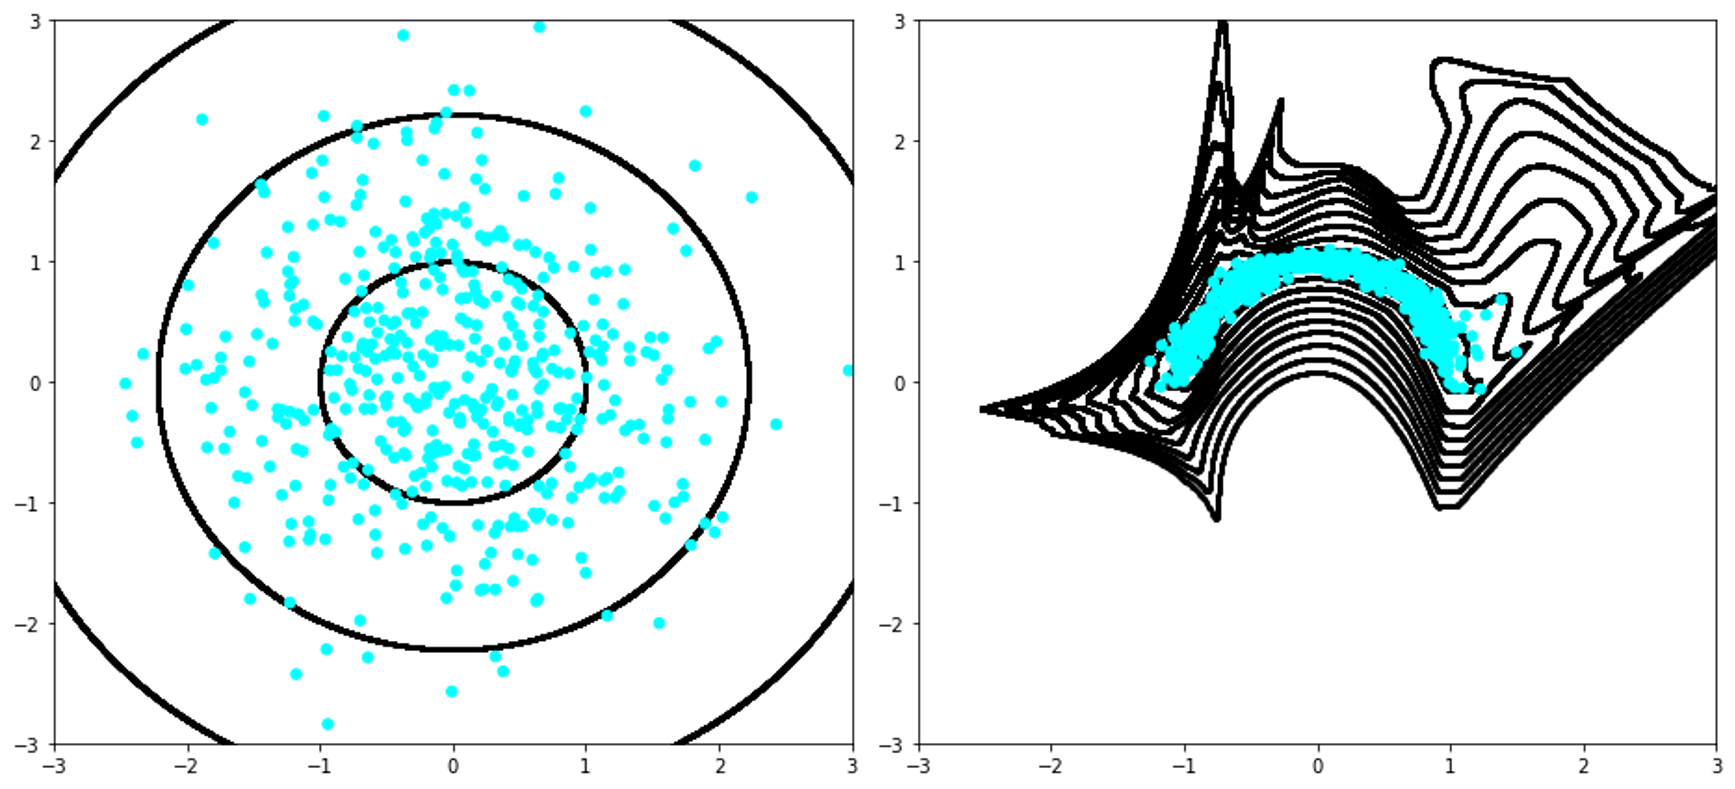
\includegraphics[width=120mm]{figs/nf_circs_cropped}
%        }
    \end{center}
    \label{fig:flow_circs}
\end{figure}

\section{Comparison Against Baselines}\label{sec:comparison-against-baselines}

Finally, our proposed probabilistic forecasting methodology (cINN) --- including recalibration, fine-tuning, and
adversarial regularization --- is compared against several baseline traditional point forecasting methods.
Comparisons are first provided against two open source state-of-the-art energy price forecasting models in literature
found in the \texttt{epf-toolbox}~\cite{epftoolbox} python library: the modified
\textit{lasso estimated auto-regressive} (EPF-LEAR) and \textit{deep neural network} (EPF-DNN) models as described in
Section~\ref{sec:baselines}.
Note, a significant downside to these models is they are only defined for single price nodes, making multi-node
forecasts significantly more expensive to obtain and the resulting forecasts would likely fail sufficiently to capture
the joint structure between node prices.
As such, only comparisons at a select few price nodes are performed.
For each price node, a single DNN model and 24 hourly LEAR models are constructed.
Univariate density forecasts for each price are obtained by marginalizing out samples from the entire joint density
forecast.
The same training and recalibration procedures previously described are implemented for both the EPF-LEAR and EPF-DNN
models, however, no rolling training or fine-tuning windows are used.
Comparisons between the CRPS of the probabilistic forecasts against the MAE of the EPF-DNN and EPF-LEAR forecasts
are shown in Table~\ref{tab:epf_comp}.
The proposed density forecasting method produces more accurate forecasts than state-of-the-art point forecasting methods.
Note, beyond greater forecast accuracy the probabilistic forecasts also captures joint structures between
price nodes and uncertainty in forecasts which non-probabilistic forecasts fail to provide.

\begin{table}[htb]
    \caption[Proposed density forecasts v.s. open-access literature point forecasts]{
        Comparison of forecast accuracy between the proposed probabilistic forecasting strategy and state-of-the-art
        point forecasting models from the $\texttt{epf-toolbox}$~\cite{epftoolbox} python library over single price
        nodes.
    }
    \begin{center}
        \begin{tabular}{||c|c|c|c||} \hline
        \diagbox{Price Node}{Model} & EPF-LEAR (MAE) & EPF-DNN (MAE) & cINN (mCRPS)  \\	% footnote symbols!
        \hline \hline
        CHICAGO HUB    & 6.622 & 6.231 & \textbf{5.341} \\ \hline
        DOMINION HUB   & 7.077 & 6.565 & \textbf{6.174} \\ \hline
        EASTERN HUB    & 7.095 & 7.526 & \textbf{6.087} \\ \hline
        NEW JERSEY HUB & 4.923 & 5.025 & \textbf{3.983} \\ \hline
        OHIO HUB       & 6.444 & 6.119 & \textbf{5.558} \\ \hline
        \end{tabular}
        \\ \rule{0mm}{5mm}
    \end{center}
    \label{tab:epf_comp}
\end{table}

Next, the proposed density forecasting methodology is compared against the commercial OPF solver.
The solver only produces point forecasts on a subset of 14 of our price nodes, thus the joint
density forecast on those specific nodes is marginalized out from the larger joint density.
Again, the MAE of the OPF forecasts is compared against the mCRPS of the probabilistic forecasts with results shown
in Table~\ref{tab:opf_comp}.
The probabilistic forecasting strategy is more accurate than the commercial, physics-based price
forecasting tool, again with the added benefit of information-rich joint probabilistic forecasts as opposed to
low-information point forecasts.

\begin{table}[htb]
    \caption[Proposed density forecasts v.s. commercial optimal powerflow solver point forecasts]{
        Comparison of forecast accuracy between our proposed probabilistic forecasting strategy and a commercial
        OPF solver point forecasting product over a subset of 14 price nodes.
    }
    \begin{center}
        \begin{tabular}{||c|c|c||} \hline
        Model & MAE (-) & mCRPS (-)  \\	% footnote symbols!
        \hline \hline
        OPF  & 6.666 &           -    \\ \hline
        cINN &   -   & \textbf{5.435} \\ \hline
        \end{tabular}
        \\ \rule{0mm}{5mm}
    \end{center}
    \label{tab:opf_comp}
\end{table}

Figure~\ref{fig:forecast_timeseries} illustrates forecasts from our joint density method and the three baseline methods
against observed DA prices on a single node over two time intervals in 2021.
Observe how the uncertainty in the probabilistic forecasts changes over time with respect to market conditions.
Also note that beyond the mean forecast and 95\% confidence intervals each forecast is a complex probability density
function as shown in Figure~\ref{fig:univar_dens}.

\begin{figure}[htbp]
    \caption[Timeseries of observed v.s. forecast prices over 2/12/21-2/17/21 and 8/13/21-8/18/21]{
        Forecasts from the proposed probabilistic forecasting methodology, EPF-LEAR, EPF-DNN, and OPF baselines
        against the true NEW JERSEY HUB DA LMPs over two five-day intervals in 2021.
        \textbf{Left:} forecasted and observed LMPs over a five-day interval during an extreme winter weather event in Texas which
        caused unprecedented price action in PJM (2/12/21-2/17/21).
        \textbf{Right:} forecasted and observed LMPs over a five-day interval in the summer (8/13/21-8/18/21).
    }
    \begin{center}
        \setlength{\fboxsep}{0pt}%
        \setlength{\fboxrule}{1pt}%
%        \fbox{
        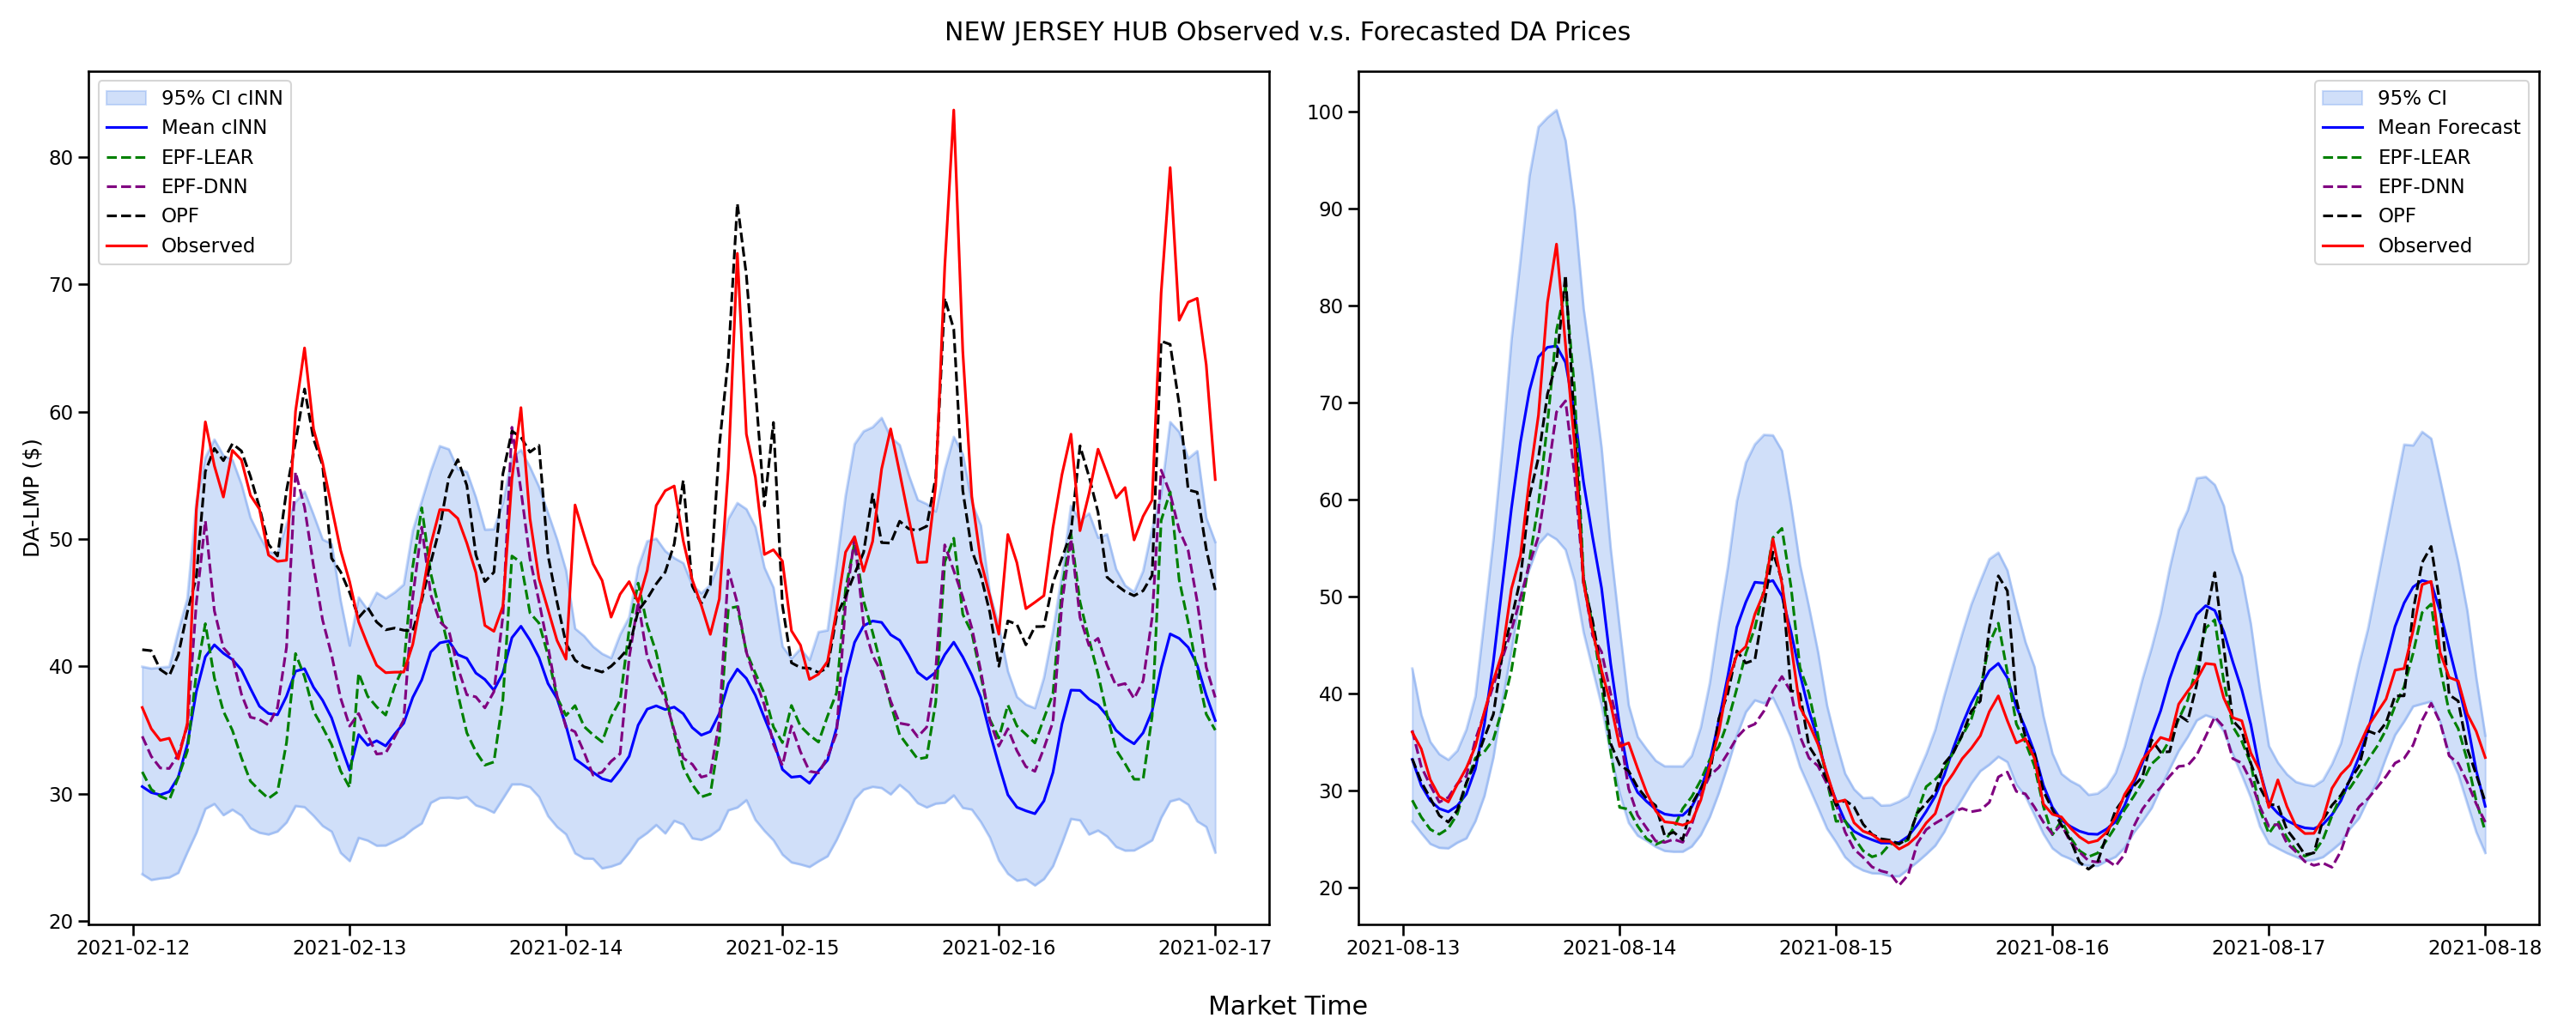
\includegraphics[width=150mm]{figs/nj_hub_ts}
%        }
    \end{center}
    \label{fig:forecast_timeseries}
\end{figure}

\begin{figure}[htbp]
    \caption[Density forecasts v.s. point forecasts v.s. observed prices on 8/13/21 hours 4, 12, 16, and 20]{
        Forecasts for the proposed probabilistic forecasting methodology and EPF-LEAR, EPF-DNN, and OPF baselines
        against the true DA prices are shown at the NEW JERSEY HUB price node at four hours on a single market-day.
    }
    \begin{center}
        \setlength{\fboxsep}{0pt}%
        \setlength{\fboxrule}{1pt}%
%        \fbox{
        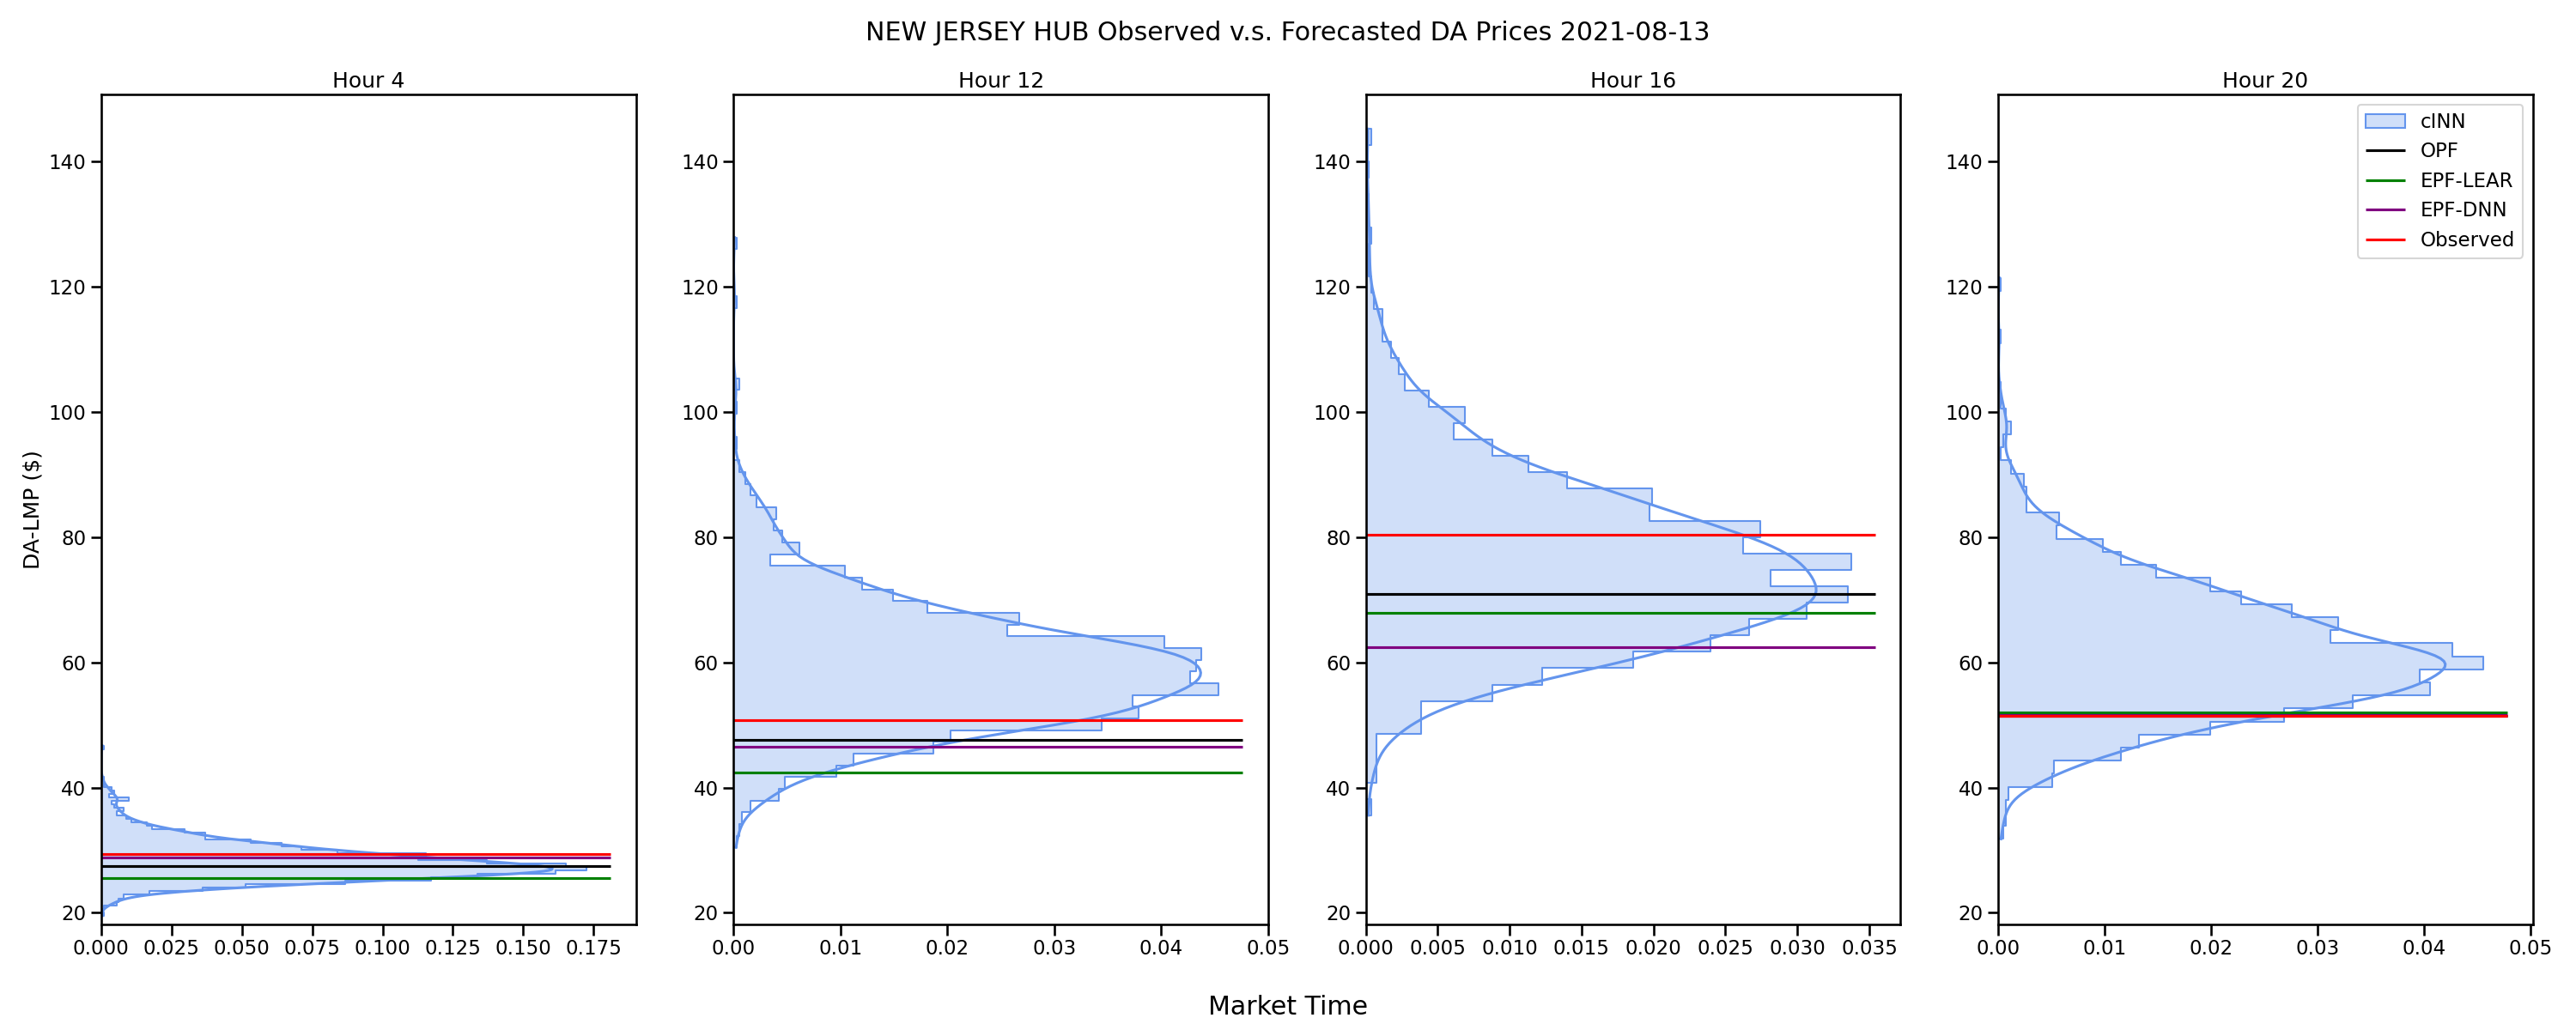
\includegraphics[width=150mm]{figs/nj_hub_densities}
%        }
    \end{center}
    \label{fig:univar_dens}
\end{figure}
